\chapter{A Practical and Scalable Software Protection enforced by TEE}
\label{chp:static-protection} 

%Here, I answer to the following question: \textbf{is a program loaded in 
%memory 
%as intended?}
%
%The answer to this question is addressed in two papers:
%\begin{itemize}
%	\item Careful-Packing: A practical and scalable anti-tampering software 
%	protection enforced by trusted computing (CODASPY 2019).
%\end{itemize}
%
%\todo{stuff from the paper}

%\section{Introduction}
%The widespread of commercial software and of potential security threats makes 
%it necessary to develop systematic 
%protection mechanisms.
%For instance, a customer could attempt to use a program 
%without paying the license fee~\cite{hacklicense}, a player might cheat in a 
%video-game~\cite{hoglund2006hacking}, or an anti-virus software can be 
%sabotaged~\cite{doubleanget} by malware.
%To achieve these goals, a common strategy is to edit the binary code of such 
%software in order to alter its logic.
%These threats are often referred to as Man-At-The-End attackers 
%(MATE)~\cite{AKHUNZADA201544}.
%Both academic researchers and commercial companies have spent an extensive 
%effort against MATE 
%threats~\cite{banescu2017detecting,ghosh2010secure,collberg2002watermarking, 
%evenbalance,vac,janusdrm}.
%The goal of the defending mechanisms is to guarantee that an attack 
%cannot change the software logic to some extent. 
%It is possible to achieve this goal in different ways, \eg through 
%anti-tampering 
%techniques~\cite{nagra2009surreptitious} or through trusted computing 
%technologies~\cite{helbig1998trusted}.
%
%Anti-tampering techniques allow a software to inspect itself and check whether 
%its code has been modified.
%We refer to those techniques as \emph{self-checking}, which literally read the 
%binary code of the protected software by using special functions called 
%\emph{checkers}.
%The checkers compute a digital fingerprint of the software bytecode and verify 
%whether that fingerprint matches a 
%pre-computed value~\cite{nagra2009surreptitious}. 
%%The latter is often referred to as \emph{self-checking}.
%On the other hand, trusted computing technologies 
%provide dedicated hardware so that the software can be executed in secure 
%containers which are physically separated from the rest of the system.
%Those containers are composed of memory regions that cannot be directly 
%read/written by other processes (either from kernel-space or from user-space).
%%It is possible to execute software and store information in the secure 
%%container such that other processes (either from kernel-space or from 
%%user-space) cannot directly interact with the protected memory.
%Trusted computing technologies are further reinforced against physical attacks 
%such as 
%flashing BIOS/firmware, page swap, or page cache 
%attacks~\cite{costan2016intel}.
%
%However, both anti-tampering and trusted computing have limitations. 
%On the one hand, purely software-based anti-tampering techniques are not 
%completely secure, since the defending mechanisms reside in an untrusted 
%memory 
%region and a determined attacker can identify and disarm such defenses.
%It is possible to harden anti-tampering techniques by using a combination of 
%additional 
%approaches~\cite{banescu2017tutorial,chen2016advanced,chang2001protecting,viticchie2016reactive}
% that raise the bar for the attackers but that do not 
%fundamentally address the problem~\cite{horne2001dynamic}.
%On the other hand, trusted computing technologies, which provide higher 
%security guarantees than purely software-based solutions, often have 
%practical limitations, e.g., software within a secure container cannot 
%directly 
%interact with the hosting 
%operating system (OS); and the secure container often has size 
%limitations~\cite{baumann2015shielding}.
%Previous works studied solutions that move part of the OS functionality inside 
%a trusted 
%region~\cite{baumann2015shielding,arnautov2016scone,tsai2017graphene},
%but they introduce further complexity %(\eg Drawbridge 
%%system~\cite{porter2011rethinking}) 
%for employing a secure interaction with the rest of 
%the world (\eg networking, file system).
%Other authors suggested protecting only portions of the 
%code~\cite{schuster2015vc3,lind2017glamdring}.
%However, these approaches do not address critical limitations such as the 
%interaction with the underlying OS, or the limited amount of memory.
%%Indeed, designing trusted containers that can handle graphical interfaces 
%%requires to rethinking the interaction container/OS.
%Limited memory makes it unsustainable to deploy all processes in dedicated 
%trusted containers.
%For instance, machines featured with Intel Software Guard eXtension 
%(SGX)~\cite{rozas2013intel} provide only a few hundred megabytes that must be 
%shared among all the running trusted containers.
%If we consider processes such as Skype or Firefox, which require around 
%$100$MB 
%each,
%we need multiple trusted containers for each process to protect.
%Therefore, this approach does not scale for multiple parallel processes.
%The introduction of SGX 2.0 allows modifying the size of a single trusted 
%container but it does not modify the maximum memory available for trusted 
%containers.

%\todo{probably starts from here}
In this chapter, we propose a technique that overcomes the limitations of both 
pure anti-tampering and trusted computing by combining both approaches.
We extend hardware security features of trusted computing over untrusted memory 
regions by using a minimal (possibly fixed) amount of code.
To achieve this, we harden anti-tampering functionality (\eg checkers) by 
moving them in trusted components, while critical code segments
(which invoke the checkers stored within a trusted module) are protected by 
cryptographic packing.
As a result, we keep the majority of the software outside of the secure 
container, this leads to three advantages:
\begin{enumerate*}[label=(\roman*)]
	\item we avoid further sophistication in communicating with the OS,
	\item we maximize the number of trusted containers issued 
	contemporaneously, and 
	\item we also maximise the number of processes protected.
\end{enumerate*}

Realizing our idea in practice is non-trivial.
Besides the self-checking functionalities, we need to carefully design other
phases of our approach such as installation, boot, and response.
The installation phase must guarantee that the program is installed properly, 
while 
the boot phase should validate that the program starts untampered. Both phases 
require us to solve the attestation problem.
The third phase, the response, is the mechanism which allows a program to 
react against an attack once it has been detected.
Moreover, trusted computing technologies, such as SGX, do not offer stand-alone 
threads 
that can run independently of insecure code. Instead, protected functionality 
needs 
to be called from (potentially) insecure code regions. As a result, such 
technologies  
do not provide \emph{availability} guarantees. 
Therefore, one design aspect of our solution is to cope with and mitigate 
\emph{denial of service} threats.
%we strengthen anti-tampering techniques because we move their sensitive code 
%inside secure containers.

As a proof-of-concept, we implemented a monitoring application
which integrates our approach. 
For this example, we opted for SGX as a trusted module. 
The application is an agent which traces user's events (\ie mouse movements 
and keystrokes) and stores the data in a central server.
We developed the monitoring agent in C++ and we deployed it in a Windows 
environment.
In our implementation, we designed the checkers to monitor those
functions dedicated to collect data from the OS, while the response was 
implemented as a 
digital fingerprint which represents the status of the client 
(\ie client secure, client tampered).
%Through this implementation we aim to show that our technique is less invasive 
%then previous ones and that the overhead in term of lines of code (LoC) and 
%benchmarks is low, tow LoCs for checker and around $5\%$ of overhead on 
%average 
%respectively.
%This implementation also helps us to illustrate how to achieve a secure 
%installation and boot phases.

To evaluate our approach, we systematically analyze which attacks can be 
performed against our approach and we show that, with the user monitoring 
application, our solution provides better protection than previous approaches. 
%In theory, our approach may suffer from just-in-time Patch \& Repair attacks, 
%where an attacker may try to bypass our protection by injecting malicious code 
%in between two unpacking/packing operations and checking. To conduct such 
%attack, 
%the attacker is required to inject the code such that it is executed without
%being detected by the checkers. 
%We show how this scenario is practically impossible without 
%controlling task scheduler.
We measure the overhead of our approach in terms of Lines of Code (LoC), 
execution time, and trusted memory allocated. We 
show that fewer than $10$ LoC are required to 
integrate our approach, while the trusted container requires around $300$ LoC.
Furthermore, the overhead in terms of execution time is 
negligible, i.e., on average $5.7\%$ \wrt the original program.
During our experiment, we managed to run and protect up to 90 instances at the 
same time.
%Finally, we will show that a single trusted container requires only $300KB$.
%Lastly, we discuss how our approach could be included seamlessly in the 
%software life-cycle.

\vspace{-0.25cm}
\paragraph{\textbf{Problem Statement:}} 
The research question we are addressing in this chapter is thus: Is it possible 
to extend trusted computing security guarantees to untrusted memory regions 
without moving the code entirely within a trusted module?

\vspace{-0.25cm}
\paragraph{\textbf{Contributions:}}In summary, the contributions of this paper 
are:

\begin{enumerate*}[label=(\textbf{\alph*})]
	\item We propose a new technique to extend trusted computing over untrusted 
	zones minimizing the amount of code to store within a trusted module.
	\item We propose a technique to mitigate \emph{denial-of-service} problems 
	in trusted computing technologies.
	\item We propose an algorithm for achieving a secure installation and boot 
	phase.
\end{enumerate*}

\section{Threat Model}
\label{ssec:back-attacker}

In a tampering attack, the goal of an attacker is to edit the code of a victim 
program~\cite{collberg2002watermarking}.
This goal can be achieved in different ways.
One way is to change the bytecode of a program before its execution, this is 
called \emph{off-line} tampering.
That is, the attacker first analyzes the binary of the program and then 
disables/removes the anti-tampering mechanisms.
The challenge for an attacker is thus to remove the anti-tampering mechanism 
without compromising the program logic.
Using tools such as debuggers or analyzers, the attacker can deduce how the 
anti-tampering protection works and disable it accordingly.
To cope with \emph{off-line} attacks, it is possible to adopt anti-tampering 
mechanisms based on digital fingerprint mechanisms.
They employ a cryptographic fingerprint of software (\eg signature, hash, 
checksum) to validate software status before the 
execution~\cite{diversig,abera2016c}.
Besides \emph{off-line} attacks, there are the so-called \emph{on-line} attacks.
In this category, the attacker aims to edit the code during the execution of 
the victim program.
Such attacks can be performed either from the kernel-space or from the 
user-space.
The key to such attacks is to synchronize the attacker and the victim process 
such that the victim code is edited in a way unnoticed by the anti-tampering 
mechanism.

In our scenario, an attacker can compromise the victim logic (\ie the bytecode) 
by using both \emph{off-line} and \emph{on-line} approaches.
%The final goal is to run the (edited) victim software in the original 
%environment.
We also consider acceptable to steal the victim software, or a piece of, as 
long as this keeps the environment unaltered.
A suitable example for our scenario is represented by distributed anti-viruses. 
This software is composed by a client-server infrastructure and they are 
commonly used in companies. 
In particular, the clients report the status of their host machine to a central 
server, and the server stores the reports and eventually notifies an intrusion.
In our example, it is possible to mount a set of attacks that will be easily 
detected.
For instance, if a client is disabled, the central server will detect the 
anomaly, similarly if an unauthorized client is installed.
If an attacker manages to steal a copy of the client software, it may be 
possible to run a tampered client in a controlled environment made ah-hoc, 
however, as long as the attacker cannot run such client in the original 
infrastructure, there is not effective damage for the companies.
%Alternatively, an attacker may achieve to run a client in an external 
%infrastructure made ad-hoc (different by the corporate one), however, in this 
%case the original corporate infrastructure will not result compromised at all.
A tampered client becomes really dangerous when the attacker manages to run 
such client in the corporate environment in order to 
%Besides all previous attempts, a serious threat is represented by an attacker 
%who manges to tamper with a client (\eg through malware) in order
allow illicit activities. In this case, the attack has to happen such that the 
central server does not recognize the anomaly.
%We designed our solution to cope with such scenarios, that will be recalled in 
%Section~\ref{sec:approach} and Section~\ref{sec:implementation_packing}.

The attacker model we consider works at user-space level; therefore, we assume 
the kernel is healthy.
Having a healthy kernel is acceptable in corporate scenarios where the machines 
are constantly checked.
Moreover, a user-space threat (\eg user-space malware, spyware) is generally 
simpler to mount than one at kernel-space.
%\todo{here}
Even though we assume having a trusted kernel, and we could have  instantiated 
our approach on the kernel itself, we opted to implement our PoC by using SGX 
in order to raise the bar for attackers that have compromised the kernel, as we 
will discuss in the following sections.
%This makes the attack more cumbersome.
We also assume the machines are not virtualized, this avoids the attacker to 
use VMX features~\cite{uhlig2005intel}.
Moreover, we assume the task scheduler is trusted, this is crucial to avoid a 
perfect synchronization of two processes (see Section~\ref{sec:just-in-time}).

To sum up, the adversary we face has the following properties:
\begin{enumerate*}[label=(\roman*)]
	\item he can analyze and change the binary \emph{off-line};
	\item he can change the \emph{on-line} memory of a victim process at 
	runtime;
	\item he cannot tamper with the task scheduler;
	\item he cannot virtualize the victim machine.
\end{enumerate*}

\section{Design}
\label{sec:approach}

%The family of solutions which guarantee the application code remains the same 
%during software execution are called \emph{anti-tampering} techniques.
Our \emph{anti-tampering technique} is an extension of the classic 
\emph{self-checking}
mechanism. In the following, we describe how we improve upon existing 
techniques with trusted computing technologies. We start with a description of 
the problem addressed and then analyze
limitations of existing approaches before explaining how our idea can help to 
limit the attacking surface of existing approaches.

\subsection{Challenges}
\label{ssect:design-theory}
%We use a simple software abstraction to illustrate the technical challenges we 
%face, and the security guarantees we desire to achieve.
In our model, a program's execution can be described as a triplet $(M,b,i)$ 
where $M$ represents the state of the program (\ie memory), $b$ is the sequence 
of instruction to execute (\ie code section) and $i$ denotes the next 
instruction to execute (\ie instruction pointer).
For simplicity, we focus on sequential and deterministic programs, whose 
instructions are executed step-by-step; however, in Section~\ref{sec:approach} 
we will discuss also multi-threading scenarios.
Each step of the program can be represented as follows:
\[ (M,b,i) \rightarrow (M^\prime,b^\prime,j), \]
where $M^\prime$ is the updated memory status, $b^\prime$ is the updated 
instruction sequence, and $\rightarrow$ is the small-step semantics of the 
program.
From a software security point of view, a program should satisfy the following 
properties:
\begin{enumerate*}[label=(\textbf{\roman*})]
	\item the next instruction $j$ must be decided uniquely by the program 
	logic (\ie $M$ and the current instruction at $i$);
	\item the program state $M'$ must be determined according to the previous 
	program state $M$, and the instruction executed $i$; %, and its code 
	%section (\ie $M^\prime=f(M,b,i)$),
	\item instructions $b$ must not change during the program execution (\ie 
	$b=b^\prime$).
\end{enumerate*}
Note that we assume that the application code is not dynamically generated, and 
that input and output operations happen through writing/reading operation in 
the memory.

Property (\textbf{i}) is related to the control flow integrity 
problem~\cite{8269390}, which is guaranteed neither by anti-tampering 
techniques~\cite{nagra2009surreptitious} nor by trusted 
computing~\cite{lee2017hacking}.
But it is tackled by tools such as~\cite{microsoftcfg,tice2014enforcing} and 
discussed in previous 
works~\cite{onarlioglu2010g,wang2010hypersafe,abadi2005control,zhang2013control,davi2014stitching}.

Property (\textbf{ii}) can be guaranteed by moving only sensitive data inside a 
trusted module and using \emph{get()}\textbackslash{}\emph{set()} functions for 
interacting with them.
This was already implemented by Joshua et al.~\cite{lind2017glamdring} in their 
Glamdring tool.
%However, the latter can be even improved by keeping all values inside untrusted
%memory regions along with a signature, and access to them by using 
%\emph{get()}\textbackslash{}\emph{set()} functions as we already outlined.
Such a solution is prone to space constraint because it keeps data within the 
trusted module (\ie an enclave).
%this can be still overcame by adopting
%\emph{get()}\textbackslash{}\emph{set()} API which 
%\todo{MO: I don't understand the last sentence}
%\feedback{FT: I tried to make it simpler}

Property (\textbf{iii}) can be implemented by moving all code inside trusted 
modules, which was the first approach 
employed~\cite{baumann2015shielding,arnautov2016scone,tsai2017graphene}.

However, simply moving all code into the trusted module has two problems.
First, a trusted module has a limited amount of memory available, and therefore 
only
certain critical sections can be executed securely.
Second, the application needs access to other OS layers to interact with the 
environment (network, peripherals).
Our approach aims to address these limitations.

A naive \emph{anti-tampering} mechanism is to run a \emph{checker} function 
over the entire code $b$ right before executing any instruction. This is 
described as follows:
\[ (M,b,i) \rightarrow check(b) \rightarrow (M^\prime,b^\prime,j), \]
where the $check()$ function verifies the integrity of the code $b$.
This approach verifies the integrity of the entire application code at each 
step. However, this is inefficient since a program must read its entire code at 
each step. Furthermore, we must protect the \emph{checker} function throughout 
the program.

In order to address space and efficiency constraints, as suggested 
in~\cite{brumley2004privtrans,singaravelu2006reducing,smith2006refactoring}, we 
may consider only certain parts of the program to be sensitive, which are 
referred to as \emph{critical sections} (CS) hereafter.
CSs include delicate parts of the software such as license checking in 
commercial products. We could thus focus on protecting only the critical part 
of the program and checking a block of instructions instead of the entire 
program (\ie CSs).
%From a practical point of view, a critical section might be a block of code or 
%longer sections of software which we aim to protect.
%After these consideration,
%We can thus reformulate the technique previously described by performing a 
%check over the critical section.
%That checking might be performed before its execution.
%This is illustrated by the following formula:
That is, instead of checking every instruction in every step, we check only the 
CSs.
Therefore, the function \texttt{check()} is executed when we encounter an 
instruction starting a CS.
This is illustrated as follows:
%\begin{align}
\begin{align}
	(M,b,i) & \xrightarrow{\text{if}~i~\in~\text{CS}} check(CS) \rightarrow 
	(M^\prime,b^\prime,j) \nonumber \\
	(M,b,i) & \xrightarrow{\text{else}} (M^\prime,b^\prime,j), \nonumber
\end{align}
where $i~\in~\text{CS}$ means the instruction \emph{i} is the beginning of a 
critical section \emph{CS} and \emph{check(CS)} checks the critical section 
$CS$.

%This model is only a generic concept of our technique, which will be fully 
%described in the following sections.
Intuitively, even though the above idea improves the efficiency of the 
anti-tampering mechanism, it is still subject to attacks. Firstly, it is 
subject to just-in-time patch \& repair. That is, an attacker could synchronize 
its actions to change the victim code right after the checking and restore the 
original code before the checker is executed again.
To conduct such an attack (without having to compromise the task scheduler), 
the attacker and the software to be protected must run as concurrent processes, 
and the attack must time its actions according to the task scheduler.
We argue that this attack is practically very challenging to carry out.
In Section~\ref{sec:just-in-time}, we discuss the feasibility of such attacks 
in more depth.
Secondly, an attacker may compromise the anti-tampering mechanisms (\ie modify 
the checkers and responses). 
Defenses against these attacks already exist.
For instance, one may employ code obfuscation on \emph{checkers} and 
\emph{responses} so that the attacker would not identify them; or design the 
\emph{checkers} and \emph{responses} such that they are strongly interconnected 
with the application code~\cite{biondi2006silver} so it is challenging to 
compromise the anti-tampering mechanisms without compromising the application 
logic; or move part of the code (\eg checkers and responses) to the 
server~\cite{viticchie2016reactive}.
These approaches are however prone to a similar threat, \ie all of them 
allocate their detection system in untrusted zones, 
and therefore, with enough time any attacker can understand and disarm these 
systems.

\subsection{Anti-Tampering based on Trusted Computing}

In this section, we will present the technical solutions to realize our 
approach in a real system.
%Realizing our approach to a real system requires us to overcome a set of not 
%trivial technical challenges, in this section we will present our solutions.
To achieve this, we require a trusted module to harden anti-tampering 
techniques.
For the sake of coherence with our proof-of-concept implementation (see 
Section~\ref{sec:implementation_packing}), we use the Intel Software Guard 
eXtension 
(SGX)~\cite{rozas2013intel} terminology.
However, it is possible to use other trusted modules (see 
Section~\ref{sec:discussion_packing}).

\begin{figure}[t]
	\centering
	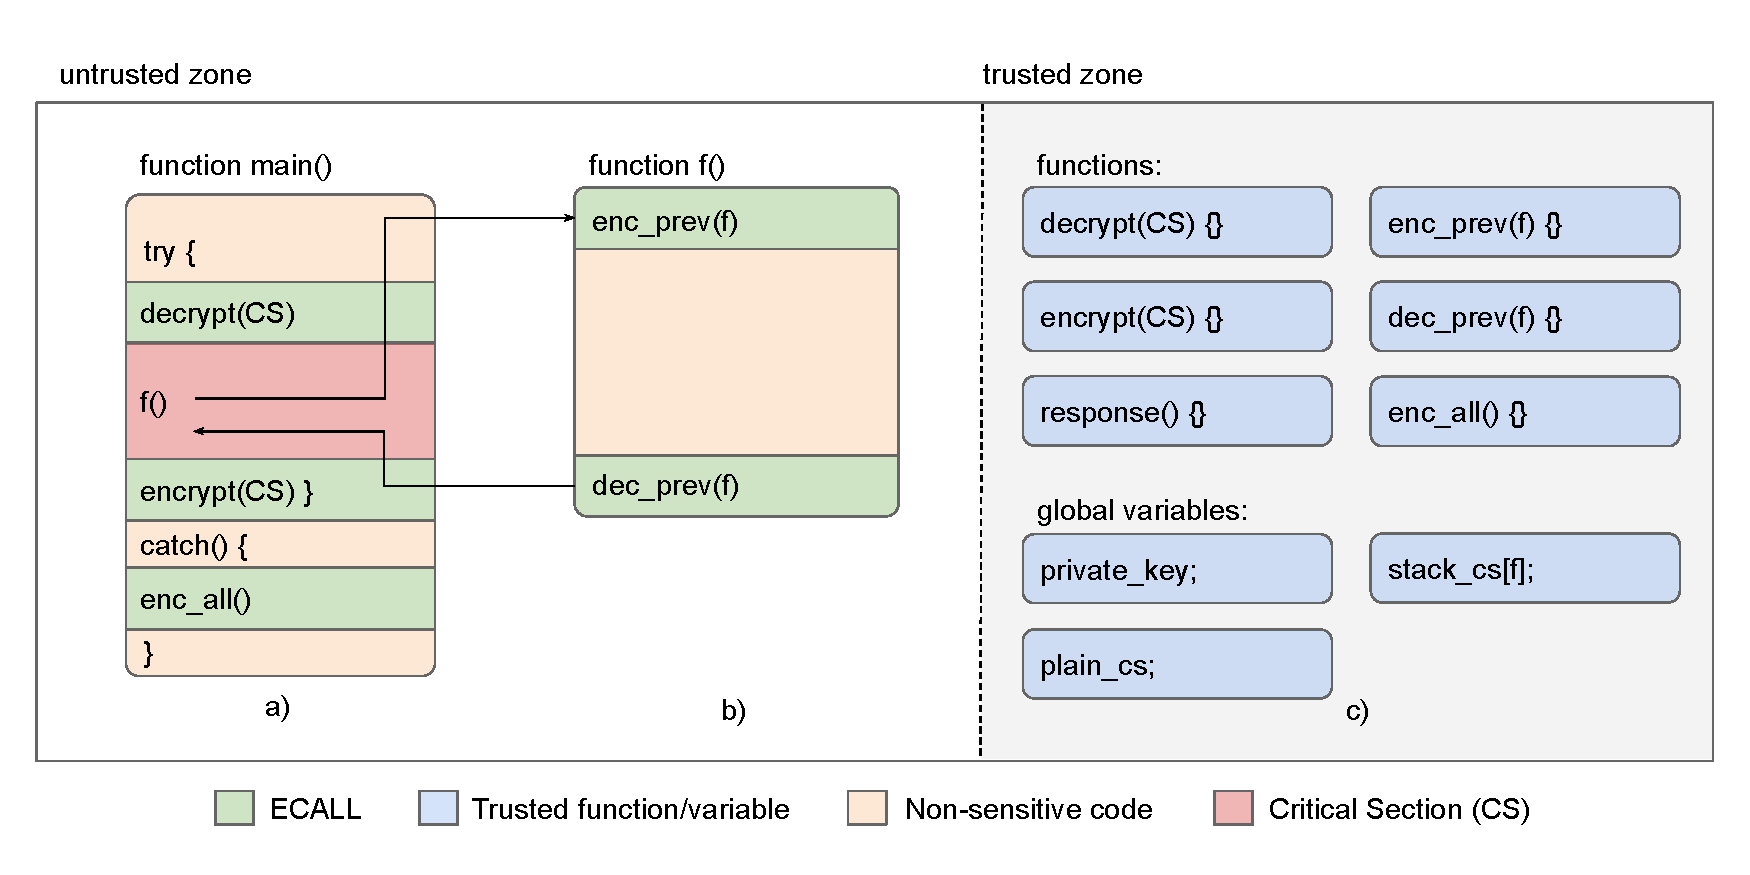
\includegraphics[width=0.7\textwidth]{fig_c3/core-all.pdf}
	\caption[Overview of single-thread schema.]{An overview of our schema for 
	single-thread applications, the memory is split in trusted and untrusted 
	zones. The trusted zone contains all methods required for our technique, 
	while in the untrusted zone we show the interaction of those methods with 
	the CSs.}
	\label{fig:core-all}
\end{figure}

Unlike previous solutions that simple ``hide'' checking functions by adopting
obfuscation or anti-reversing 
techniques~\cite{banescu2017tutorial,chang2001protecting,chen2016advanced,viticchie2016reactive},
 we store
code relevant to the anti-tampering mechanism in a trusted module (\ie an 
enclave),
through which we monitor and react to attacks conducted on
the untrusted memory region.
Saving anti-tampering mechanisms within trusted containers is significantly 
different from previous purely software-based solutions since an attacker 
cannot directly tamper with them.
This is illustrated in Figure~\ref{fig:core-all}, which presents an overview of 
our technique.
In detail, a given application is divided into two zones: an untrusted zone (on 
the left side) and a trusted zone (on the right side).
The untrusted zone contains the entire application code,
whereas the trusted zone contains all functions and global variables employed 
by our anti-tampering technique, such as \emph{checkers} and \emph{responses} 
(shown in blue).
The untrusted zone is further divided into different regions: the CSs which we 
aim to protect (shown in red), the non-sensitive blocks (shown in pale yellow) 
and the code for calling the trusted functions in the trusted zone (shown in 
green).
We also included three labels (\ie a, b, and c) to identify specific regions 
that will be used ahead in the discussion.
By using this structure, we can check the status of the untrusted zone by being 
inside the trusted zone.
%FLAVIO: that's not true anymore :D
%Note that we keep the same color convention for describing next figures.

\paragraph{\textbf{Critical Section Definition}}
A CS is any continuous region of code which is surrounded by two instructions, 
respectively labeled as \emph{CS\_Begin} and \emph{CS\_End}, and that satisfies 
the following rules:

\begin{enumerate}
	\item\label{vcs:function} \emph{CS\_Begin} and \emph{CS\_End} must be in 
	the same function.
	\item\label{vcs:sequence} For each program execution, \emph{CS\_Begin} is 
	always executed before \emph{CS\_End}.
	\item\label{vcs:noexit} Every execution path from a \emph{CS\_Begin} must 
	reach only the corresponding \emph{CS\_End}.
	\item\label{vcs:nooverlap} Every execution path which connects 
	\emph{CS\_Begin} and a \emph{CS\_End} must not encounter other 
	\emph{CS\_Begin} instructions.
	\item A CS cannot contain try/catch blocks
	\item We consider function calls from within a CS as atomic,	\ie we do 
	not consider the called function as a part of the CS.
	\item\label{vcs:loops} The loops contained by a CS must be bounded to a 
	known constant.
\end{enumerate}
Points~(\ref{vcs:sequence}) and~(\ref{vcs:noexit}) can be implemented by using 
a forward analysis~\cite{moller2012static} of all possible branches from 
\emph{CS\_Begin} to \emph{CS\_End}, and considering all function calls as 
atomic operations.
We also desire that a CS contains only unwinding loops to minimize the time in 
which a CS is plain.
The other points are simply static patterns.
The above rules are implemented by static analysis at compilation time.
If a CS does not satisfy one of those requirements, the compilation process is 
interrupted.
Therefore, we assume having only valid CSs at runtime.

In order to maintain the application stable, and to reduce the attacker 
surface, we desire that at most one CS remains decrypted (plain) during each 
thread execution.
This is achieved by introducing a global variable, called \emph{plain\_cs}, 
within the trusted zone (as illustrated in Figure~\ref{fig:core-all}-\text{c}).
The variable \emph{plain\_cs} indicates which CS is currently decrypted.
Also, as we will illustrate later, the value of \emph{plain\_cs} is updated by 
\texttt{encrypt()} and \texttt{decrypt()} functions.
%This indicates the plain CS, if any, and it is updated only by 
%\texttt{decrypt()} and \texttt{encrypt()} functions.
%More precisely, \texttt{decrypt()} sets the variable to the CS passed as 
%argument, while \texttt{encrypt()} sets the variable to \emph{Null}.
%This helps us to keep the program in a stable state and to reduce the attack 
%surface to only one CS at the time.
%Next techniques are therefore built by taking in consideration all CS as 
%\emph{valid}, and the global variable \emph{PLAIN\_CS}.
For sake of simplicity, we describe the following techniques by considering 
only single-thread programs.
While we extend our approaches to multi-threading programs at the end of this 
section.

%\begin{figure}[t]
%	\centering
%	\begin{subfigure}[t]{.32\textwidth}
%		\centering
%		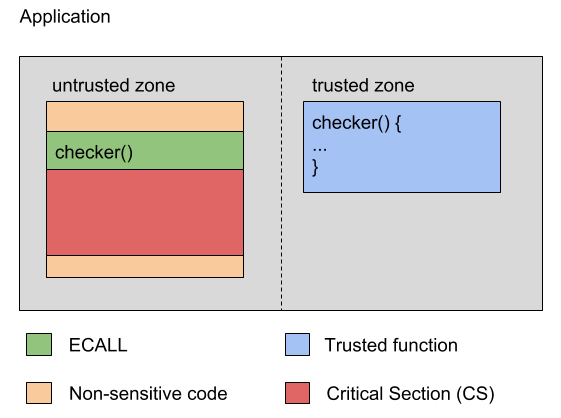
\includegraphics[width=\textwidth]{fig_c3/core-prototype}
%		\caption{Protection prototype.}
%		\label{fig:core-prototype}
%	\end{subfigure}
%	\qquad
%	\begin{subfigure}[t]{.4\textwidth}
%		\centering
%		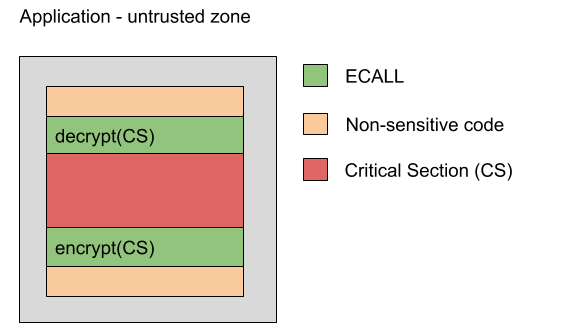
\includegraphics[width=\textwidth]{fig_c3/core-general}
%		\caption{Packaging algorithm.}
%		\label{fig:core-general}
%	\end{subfigure}
%	\caption{\todo{FT: very ugly!}}
%\end{figure}

%\begin{subfigure}[t]{0.5\textwidth}
%\centering
%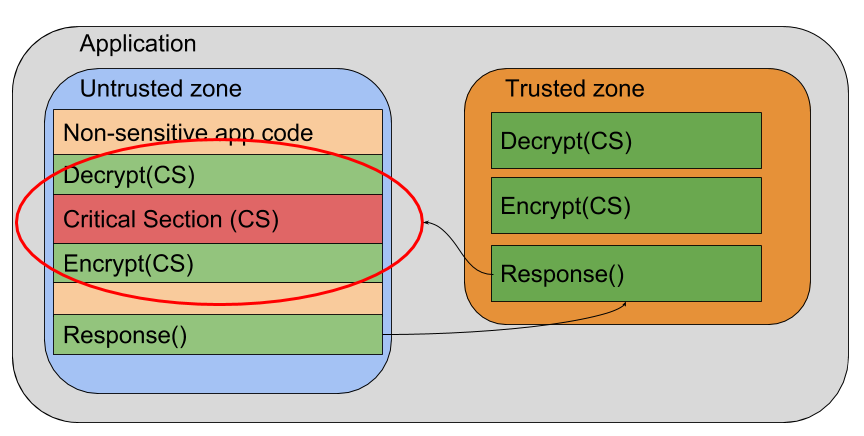
\includegraphics[width=0.5\textwidth]{fig_c3/core-response}
%\caption{Heartbeat algorithm.\todo{maybe remove it}}
%\label{fig:core-response}
%\end{subfigure}

\paragraph{\textbf{Overcoming Denial of Service Issues}}
Even if a trusted function is protected from being tampered with, usually 
trusted computing components do not provide availability guarantees, in the 
sense that the code in the trusted zone must be invoked externally.
We overcome this limitation by employing \emph{packing}~\cite{ugarte2016rambo}, 
a technique which is often used by malware to hide its functionality, combined 
with a heartbeat~\cite{ghosh2010secure}. %, which is depicted in 
%Figure~\ref{fig:sc-1p}.
Our intuition is to force the untrusted zone to call trusted functions in order 
to execute application logic.
This configuration is depicted in Figure~\ref{fig:core-all}-\text{a}.
In the beginning, CSs are encrypted (red shape). Therefore an attacker cannot 
directly change CSs' content, and the code cannot be executed unless unpacked.
%The block will be decrypted only for a small amount of time.
Each CS is surrounded by calls to two functions, which are called 
\texttt{decrypt()} and \texttt{encrypt()}.
In our design, \texttt{decrypt()} and \texttt{encrypt()} functions has the role 
of \emph{checkers}.
Those functions take a CS identification (\eg CS address) as an input, then 
they apply cryptographic operations to the CS by using a \texttt{private key}. 
The \texttt{private key} is stored inside the trusted module (see 
Figure~\ref{fig:core-all}-\text{c}).
The first call (green shape) points to
the \texttt{decrypt()} function which performs three operations:
\begin{enumerate*}[label=(\roman*)]
	\item it decrypts the CS,
	\item it sets \emph{plain\_cs} to CS, and
	\item it performs a hash of the code to check the CS integrity.
\end{enumerate*}
Once this checker is executed, the CS contains plain assembly code that can be 
processed.
As a result, the untrusted zone \emph{must} call the checker in order to 
execute the CS's code.
%After the CS, a second call to the second checker (green shape) points to the 
%\texttt{encrypt()} function which performs three operations:
After the CS, a second call (green shape) points to the \texttt{encrypt()} 
function which performs three operations:
\begin{enumerate*}[label=(\roman*)]
	\item it encrypts the CS,
	\item it sets \emph{plain\_cs} to \emph{NULL}, and
	\item it performs a hash of the code to check the CS integrity.
\end{enumerate*}
%As for the \texttt{decrypt()} function, this also performs a hash to check the 
%CS integrity.
%In our design, \texttt{encrypt()} and \texttt{decrypt()} functions has the 
%role of \emph{checkers}.
Note that \texttt{decrypt()} and \texttt{encrypt()} are considered as atomic. 
These functions are used as primitive to build more sophisticated mechanisms 
later.
We illustrate the runtime packing algorithm in Figure~\ref{fig:dec1}.
In the beginning, the CS is encrypted (\ie $E[CS]$) while the 
\texttt{decrypt()} function is executed  (Figure~\ref{fig:dec1}-\text{1}). 
After the decryption phase, the CS is plain (white color) and it is normally 
executed (Figure~\ref{fig:dec1}-\text{2}).
Finally, the \texttt{encrypt()} function is executed and the CS gets encrypted 
again (Figure~\ref{fig:dec1}-\text{3}).

Together with the packing mechanism already explained, we employ a parallel 
heartbeat as a response, which is depicted in 
Figure~\ref{fig:core-all}-\text{c}.
The heartbeat is implemented by calling a \texttt{response()} function which 
resides within the trusted zone.
The response's duty is to select a random CS and validate its hash value along 
with its respective decrypt and encrypt function calls, the outcome of this 
check is an encrypted packet shipped to a server that validates the application 
status.
The heartbeat does not prevent software tampering, it is a \emph{responsive} 
strategy to alert a central system about an attack.
To implement a heartbeat, it is possible to adopt different strategies, \eg we 
can set a dedicated thread which is risen according to a time series, or else 
we can merge the heartbeat with a communication channel between the client and 
the server (as we opted in our proof-of-concept application).

\begin{figure}[b]
	\centering
	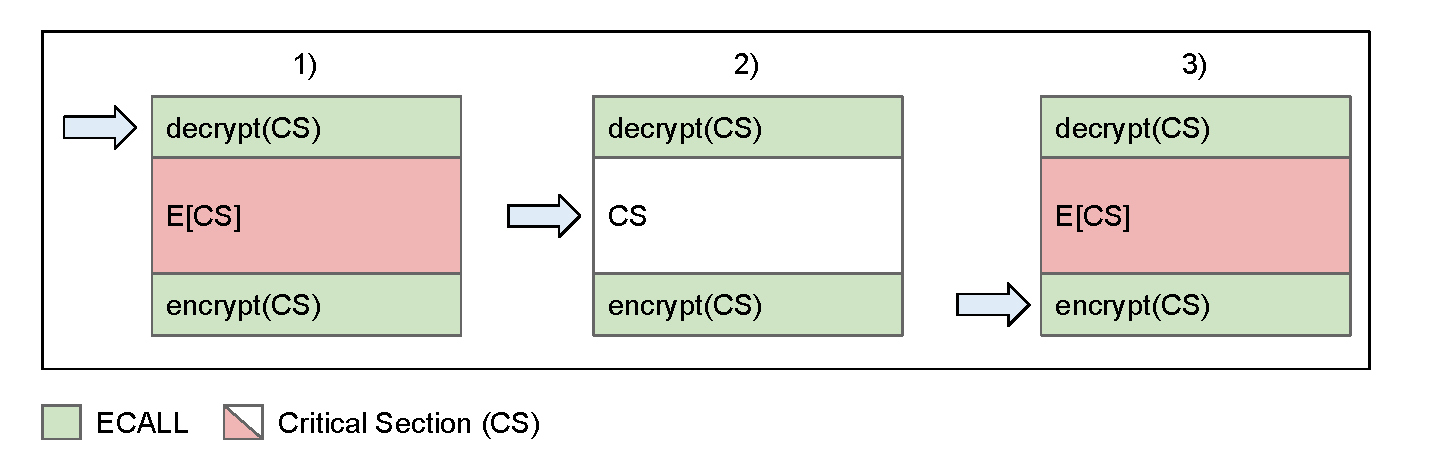
\includegraphics[width=0.7\textwidth]{fig_c3/dec1.pdf}
	\caption{Packing mechanism of our schema.}
	\label{fig:dec1}
\end{figure}

%The packaging system described since now requires further sophistications in 
%order to be employed in modern softwares.
%Since modern languages allow a developer to use software patterns such as 
%recursion or exceptions,
%we must guarantee that a CS is always encrypted before a \texttt{decrypt()} 
%function is called, and that is encrypted again after the respective 
%\texttt{encrypt()} function.
%In order to explain how we guarantee this property, we introduce the concept 
%of \emph{valid Critical Section}.
%In the following, we describe our solutions; however, this require us to 
%define which CS are considered valid.
%From this consideration, we state our third challenge:

\paragraph{\textbf{Function Calls and Recursions}}
Since we allow a CS to host function calls, a CS might remain plain after a 
call. This potentially increases the attacker surface.
To mitigate this issue, we desire that a CS is encrypted once the control 
leaves the CS itself, and decrypted again right after.
This is achieved by introducing two new functions, namely \texttt{enc\_prev(f)} 
and \texttt{dec\_prev(f)}, which are handled by the trusted module, as 
described in Figure~\ref{fig:core-all}-\text{b}.
%Their interaction with the rest of the system is summarized in 
%Figure~\ref{fig:callfunction}\todo{FT: think if we really need a picture for 
%this..maybe not}.
At compilation time, we instrument all functions that are directly called from 
within a CS by adding a function call toward \texttt{enc\_prev(f)} in their 
preamble, and toward \texttt{dec\_prev(f)} for each of its exit point (\ie 
return operation).
Both \texttt{enc\_prev(f)} and \texttt{dec\_prev(f)} functions require a 
parameter \texttt{f}, this parameter identifies which is the function that 
calls \texttt{enc\_prev(f)} and \texttt{dec\_prev(f)}.
Since several CSs can call the same function \texttt{f}, we introduce a stack 
for each function \texttt{f} to handle these cases, as depicted in 
Figure~\ref{fig:core-all}-\text{c}.
These stacks are global variable inside the trusted module, we identify the 
stack for the function \texttt{f} as follows:
$$
stack\_cs[f] = \text{stack<CS>}().
$$
%Moreover, the functions \texttt{encrypt()} and \texttt{decrypt()} edit 
%\emph{plain\_cs} variable. More precisely \texttt{encrypt()} function sets 
%\emph{plain\_cs} with the current CS, while \texttt{decrypt()} sets 
%\emph{plain\_cs} to \emph{NULL}.
The \texttt{enc\_prev(f)}, \texttt{dec\_prev(f)} functions and the 
\texttt{stack\_cs[f]} interact through each other in the following way.
Once \texttt{enc\_prev(f)} is called, it identifies whether the control comes 
from a CS by checking the global variable \emph{plain\_cs}.
If it is the case, the function performs two operations: 
\begin{enumerate*}[label=(\roman*)]
	\item it pushes \emph{plain\_cs} in \texttt{stack[f]}, and
	\item it calls \texttt{encrypt(plain\_cs)}.
\end{enumerate*}
Therefore, after calling \texttt{enc\_prev(f)} the system reaches this status:
\begin{enumerate*}[label=(\roman*)]
	\item the outer CS is encrypted (and thus protected),
	\item \emph{plain\_cs} is set to \emph{NULL}, and
	\item the thread is ready to handle a new CS.
\end{enumerate*}
Similarly, once the control leaves the function \texttt{f}, the epilogue calls 
\texttt{dec\_prev(f)}.
This function performs two operations:
\begin{enumerate*}[label=(\roman*)]
	\item it pops the last CS from \texttt{stack[f]} into \emph{plain\_cs}, and
	\item it restores the previous CS status by calling 
	\texttt{decrypt(plain\_cs)}.
\end{enumerate*}
As a result, the control can safe pass to the outer CS.
In the opposite scenario, once the control enters in the function \texttt{f} 
and the \emph{plain\_cs} is set to \emph{NULL}, it means that the function 
\texttt{f} was not called by a CS; and therefore, \texttt{enc\_prev(f)} and 
\texttt{dec\_prev(f)} do nothing.
Stacks allow us to handle recursions, if the function \texttt{f} is 
repetitively called, we trace all previous CSs.

%\begin{figure}[t]
%	\centering
%	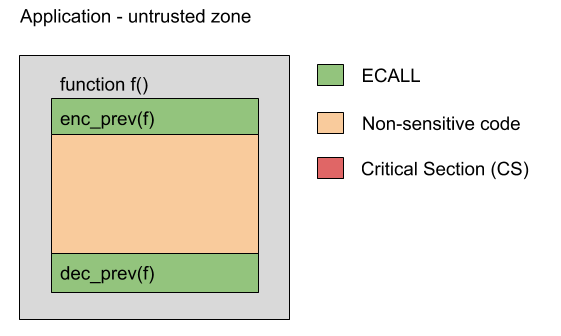
\includegraphics[width=0.45\textwidth]{fig_c3/core-callfunction}
%	\caption{Function call, when the control enters in a function, the system 
%tries to encrypt the previous vCS}
%	\label{fig:callfunction}
%\end{figure}

%This solution allows us to totally encrypt the vCS after the control leaves 
%it; other settings could

%Modern program languages, like C++, allow a user to raise exceptions in order 
%to handle unpredictable program behaviors.
%These mechanism might bring our anti-tampering system to an unstable 
%situation, \eg an exception risen in the middle of a CS will leave the CS 
%it-self decrypted.
%This introduces our last challenge:
%\begin{description}
%	\item [(C5)] How do we handle exception?
%\end{description}
\paragraph{\textbf{Exceptions within Critical Section}}
%Modern program languages, like C++, allow a user to raise exceptions in order 
%to handle unpredictable program behaviors.
%These mechanism might bring our anti-tampering system to an unstable 
%situation, \eg an exception risen by a CS will leave that CS decrypted.
We can handle exceptions from within a CS by introducing a new function, namely 
\texttt{enc\_all()}, which is handled by the trusted module, as described in 
Figure~\ref{fig:core-all}-\text{c}.
This function is an alias for \texttt{encrypt(plain\_cs)}.
That is, we wrap any CS with a try/catch block at compilation time, as 
described in Figure~\ref{fig:core-all}-\text{a}.
The exception block is made such that
\begin{enumerate*}[label=(\roman*)]
	\item to catch all exceptions, 
	\item to run \texttt{enc\_all()},
	\item to throw the exception again.
\end{enumerate*}
In this way, we restore the anti-tampering mechanism as soon as an exception 
appears. 
Thus, after an exception, we encrypt all the plain CSs and the application can 
continue normally.
Note that the \emph{response} function has to be extended in order to protect 
the \emph{catch} block,
or else, an attacker might raise an exception in order force a CS to be 
plain\footnote{We do not deal with runtime attacks to exception handlers, such 
as SEH, since they do not belong to anti-tampering problems.}.

%\paragraph{\textbf{Network protection}}
%An advanced attack can be brought right after the \emph{decryption} function 
%is executed.
%At this point, an attacker can remove invocations to any trusted functions in 
%enclaves and keep the plain code correctly decrypted.
%To avoid this type of attacks we employed a random network of checkers.
%More precisely, each \emph{decryption} function randomly checks another block 
%of code beside itself, namely \emph{external block}.
%Also, that function verifies the relative \emph{encryption} and 
%\emph{decryption} functions call of the \emph{external block}.
%The \emph{external block} is randomly decided every time a \emph{decryption} 
%function is called. The decision is taken inside the enclave by using 
%\texttt{sgx\_read\_rand} function that can generate a random number in a 
%secure 
%fashion.

\paragraph{\textbf{Multi-threading programs}}
%\todo{FT: maybe move it into extended version}
We can extend the previous techniques in order to handle parallel computation, 
this is possible because some trusted computing technologies allow 
multi-threading programming, like SGX (see Section~\ref{ssec:sgx-core-design}).
To achieve multi-threading, we maintain a \emph{plain\_cs} and a 
\texttt{stack\_cs[f]} for each thread.
%This allow us to maintain an independent status for each thread.
Moreover, we introduce a counter for each CS. % -- namely \emph{[CS]}.
These global variables represent the number of threads which are executing a CS 
in a specific moment.
In the beginning, the CSs' counters are set to \emph{zero}.
Then, they are increased and decreased by \texttt{decrypt()} and 
\texttt{encrypt()} functions respectively.
%These counters are used to understand whether a CS is under execution by some 
%thread.
%In case a CS is already decrypted (\eg $TOKEN[CS] > 0$), \texttt{decrypt()} 
%does not apply any algorithm, but it just increases the counter.
%On the other hand, if a CS is used by more than one thread  (\eg $TOKEN[CS] > 
%1$), \texttt{encrypt()} does not modify that CS, but it just decreases the 
%counter.

%\vspace{3mm}
%The entire pseudo-code of all functions described since now is included in 
%Appendix~\ref{appendix}.
%As discussed before, our approach is still theoretically prone to patch \& 
%repair attacks which will be discussed in Section~\ref{sec:experiment}, and 
%are 
%practically unlikely to succeed.
%Another problem which deserves attention is the loading of key for the 
%packaging/de-packaging algorithm. This is overcame by a secure booting phase 
%which will be discussed in the following paragraphs.

%FT: removed because already described before
%\paragraph{\textbf{Response by using Heartbeat}}\todo{FT: I think we can 
%remove it!}
%
%Since our approach is meant to be implemented in a client-server 
%infrastructure, we employed an heartbeat packet as response (more details 
%about 
%architecture in~\ref{lbl:architecture}).
%The purpose of heartbeat is twofold. First, it needs as proof to the server 
%that client is running. Second, it verifies code integrity of the client.
%This last properties is achieved by a challenge between sever and client, in 
%our assumptions client and server share the same key.
%
%The heartbeat can be implemented as periodically communication between client 
%and server, or as signature into the normal communication.
%\todo{fig}

\paragraph{\textbf{Ensuring a Secure Booting Phase}}
Our approach requires that the program has a secure booting phase, which means 
having the following assumptions for the
\emph{encrypt}, \emph{decrypt} and \emph{response}: the key for crypto 
algorithms must be loaded in a secure way together with a table which describes 
where the CSs are located (\ie their address and length) with their hash values.
We refer to this table as \emph{block table}.
We assume a trusted loading of this information by adopting SGX sealing and 
attestation mechanisms.
Those mechanisms ensure to store information on a disk or to establish a secure 
channel with other enclaves within the same machine (\ie local) or with a 
remote one (\ie remote) in a trusted way.
We detail sealing and attestation in Section~\ref{ssec:sgx-remote-attestation}.

%\subsection{New Enclave Interface}
%\todo{FT: I propose to remove it}
%\todo{FT: that's a temporary location/title. I will change it later}
%
%Goal: \textbf{for each thread, we allow at most one decrypted critical section 
%at time}.
%
%How to: all functions called from inside a CS has at preamble and trailer a 
%call to ENC\_PREV(L) and DEC\_PREV(L) respectively.
%L indicates the function called, these functions handle the previous CS in 
%case the call starts from there, or else they just do nothing.
%\todo{FT: explain practical algorithm}
%
%Our algorithm interface expose these functions:
%
%\begin{description}
%	\item[DEC(CS)] this function decrypt the critical section CS.
%	\item[ENC(CS)] this function encrypt the critical section CS.
%	\item[DEC\_PREV(L)] this function decrypt the previous critical section 
%which belongs to lelve L, if any.
%	\item[ENC\_PREV(L)] this function encrypt the previous critical section 
%which belongs to lelve L, if any.
%	\item[ENC\_ALL()] this function encrypt all plain critical sections, it is 
%needed to handle exceptions and signals.
%\end{description}
%
%This set of functions help us to handle any function calls within any CS, and 
%also recursions.
%As result we have a smaller attack surface.
%
%\begin{figure}[t]
%	\centering
%	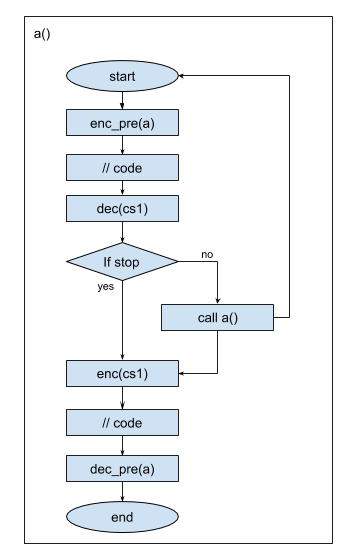
\includegraphics[width=0.5\textwidth]{fig_c3/recursivefunction}
%	\caption{Recursive function example\todo{FT: I propose to remove it}}
%	\label{fig:recursivefunction}
%\end{figure}
%
%\subsection{Critical Sections}
%\todo{FT: I propose to remove it}
%In our definition, a critical section can be any portion of code,
%therefore, they can include control flow instructions such as
%branch conditions, loops, and function calls.
%This makes challenging to implement a
%packaging algorithm which keeps the program stable and, at the same time,
%guarantees the security properties stated before. 
%For instance, a critical section which has a long execution time (\ie it 
%contains loops)
%can increase the chance of an attacker to bring a patch \& repair attack,
%or else, a recursive function, which contains a critical section, can call 
%itself 
%and then attempts to decrypt twice its own critical section.
%
%These problems can be overcome by applying our packaging approach
%to each basic block of a critical section.
%In this way, the attack surface is restricted at each single basic block,
%while, in case of function calls, each basic block is encrypted before the 
%control flow leaves the function itself.
%%However, in our proof-of-concept application described in 
%%Section~\ref{sec:implementation_packing}, we do not support
%%packaging at single basic block, even if it is possible to extend our work to 
%%support that like in~\cite{shih2017t,seo2017sgx}.
%
%\subsection{Validation of Critical Sections}
%\todo{FLAVIO: That's part of my email}
%Problem statement: how is it defined a valid Critical Section?
%
%
%Generally speaking, a critical section is manually defined by the user. 
%Therefore, it might be any random code region within a program.
%
%That's why I would define which requirements a critical section must meet in 
%order to be valid.
%
%Then, we can propose how to implement these conditions to validate all CSs at 
%compilation time.
%
%
%Critical Section definition:
%
%A critical section is any continues portion of code which is identified by two 
%instructions, namely \emph{CS\_Begin} and \emph{CS\_End}.
%
%
%Valid Critical Section definition:
%
%A valid Critical Section is a Critical Section which its \emph{CS\_Begin} and 
%\emph{CS\_End} satisfy the following rules:
%
%\begin{enumerate}
%	\item \emph{CS\_Begin} and \emph{CS\_End} must lean within the same 
%function.
%	\item For each program execution, \emph{CS\_Begin} is always executed 
%before \emph{CS\_End}.
%	\item Every execution path which starts from a \emph{CS\_Begin} must reach 
%the same \emph{CS\_End}.
%	\item It is not possible to define two consecutively \emph{CS\_Begin} or 
%\emph{CS\_End} (not CS overlapping) (I ask help to define this rule please :))
%	\item Every function call within a CS is considered as an atomic operation.
%\end{enumerate}
%
%Also, this analysis makes me think about two aspects of the program:
%
%\begin{enumerate}
%	\item how do we handle exceptions? If the critical section raises an 
%exception, this will interrupt the normal flow of the program. I have to find 
%out how to manage it. Every CS is wrapped with a try catch, in case of 
%exception we encrypt back the CS (all the CS) and we raise the exception
%	\item how do we handle signals? An operative system can raise a signal, we 
%should intercept it and react accordingly. I need some help in this as well. 
%Same as exception
%\end{enumerate}
%
%\todo{FLAVIO: keep trace the list of decrypted CSs for each thread + introduce 
%ENCRYPT\_ALL function which encrypts back all CS let open!}
%
%In both cases we have to understand whether a critical section is decrypted 
%and, in case, encrypt it again. But I don't know how.
%
%\subsection{Exceptions Handling}
%\todo{FT: just a note}
%After having identify a valid critical section, that one is wrapped in a 
%try/catch block.
%In this way, if the critical section, or some function called by this one, 
%raise an exception, we can catch it and performs a ENCRYPT\_ALL() to make 
%every 
%CS secure again.

\section{Implementation}
\label{sec:implementation_packing}
In this section, we describe a proof-of-concept implementation of our 
anti-tampering
technique, whose architecture is depicted in Figure~\ref{fig:architecture}.
The application is composed by a central server that handles a set of clients 
which are spread over a network.
%\todo{SJ: some background, in particular, the motivation of the application is 
%needed in order to set the stage.}
Each client is a monitoring application that traces user's activities (\ie 
keystrokes and mouse traces) and sends the
data to the central server.
As a trusted module, we opted for the Intel Software Guard eXtension 
(SGX)~\cite{rozas2013intel}, however, it is possible to use other solutions 
that involves the kernel (\eg TPM~\cite{tpm-isoosi}).
We deployed the architecture in a Windows environment.
Through this application we describe the specific technical solutions we 
adopted for the client, and how we implemented installation phase, boot phase, 
and response. 
%In the end, we propose a development framework to deploy our technique to any 
%application.
\begin{figure}[t]
	\centering
	\begin{subfigure}[t]{0.45\textwidth}
		\centering
		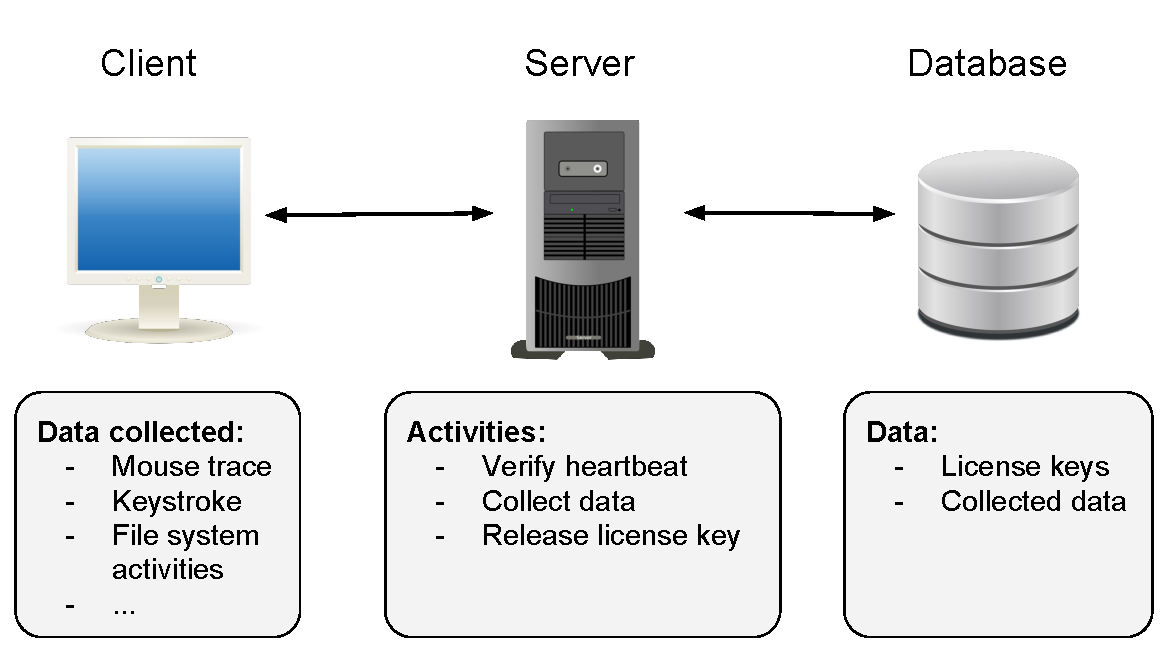
\includegraphics[width=\linewidth]{fig_c3/architecture.pdf}
		\caption{The architecture of proof-of-concept program. The client is a 
		monitoring agent which collects user's activities, the server handles 
		clients, and the database stores collect data and license keys.}
		\label{fig:architecture}
	\end{subfigure}
	\hfill
	\begin{subfigure}[t]{0.45\textwidth}
		\centering
		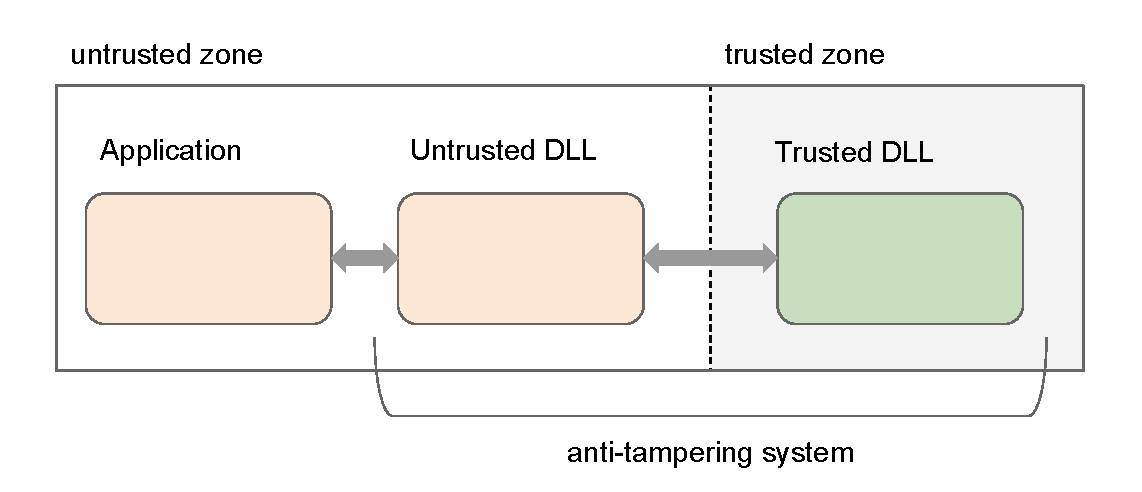
\includegraphics[width=\textwidth]{fig_c3/clientarchitecture.pdf}
		\caption{The software organization of the client.}
		\label{fig:clientarchitecture}
	\end{subfigure}
	\caption{Careful-Packing architecture.}
\end{figure}

\subsection{Client}
We describe the internal structure of the client in order to clarify some 
practical implementation strategies.
We developed this application in C++ and we deployed it on Windows machines.
For sake of simplicity, we did not implement Address Space Layout Randomization 
(ASLR)~\cite{snow2013just}, however, it is possible to deduct the right address 
offset by employing a Drawbridge system~\cite{porter2011rethinking}.

\paragraph{\textbf{Software Architecture}}
The client is formed by three modules: the main program, and two dynamic linked 
libraries (DLL) namely untrusted DLL and trusted DLL. % which are used to 
%integrate our technology into the main program.
This architecture is depicted in Figure~\ref{fig:clientarchitecture},
the application communicates with the untrusted DLL to call the functions 
described in Section~\ref{sec:approach}.
The untrusted DLL works together with the trusted DLL (\ie the enclave) to 
handle the whole anti-tampering technique.
We choose this architecture to
simplify the integration of our anti-tampering system.
In this way, the developer can focus on the main program
and integrate the anti-tampering system later.
Each component of the architecture is described as follows:
\begin{itemize}
	\item \textbf{Application:} this is the client that we aim to enforce. 
	Natively, 
	it contains all the functionalities for collecting information from the 
	underline OS and ship them to the server.
	\item \textbf{Untrusted DLL:} this contains the untrusted functions for 
	interacting with the enclave. Also, it keeps track of the status of the 
	enclave (\ie enclave pointer) and exposes routines procedures.
	\item \textbf{Trusted DLL (enclave):} this is the enclave. It contains the 
	trusted functions described in Section~\ref{sec:approach} (\eg checkers, 
	response) along with some extra routine functions (\ie installation and 
	boot).
\end{itemize}

\paragraph{\textbf{Critical Section Definition}}
%As we introduced before, one of the purposes of anti-tampering techniques is 
%to protect critical software sections which are crucial for the software logic.
Since this client is a monitoring agent, we identify as CSs those
functions used to collect the information issued by the OS:
\texttt{PAKeyStroked}, which collects keystroked, and its twin 
\texttt{PAMouseMovement},
which collects mouse events.
These functions are callback risen by the OS along with the relative event 
information.
For sake of simplicity, we trust in argument passed by the OS.
The main duties of these functions are:
\begin{enumerate*}[label=(\roman*)]
	\item collecting the data,
	\item crafting a packet with the data collected,
	\item signing the packet, and finally
	\item shipping it to the server.
\end{enumerate*}
Since in our implementation we required only integrity, we implemented a 
digital fingerprint.

\paragraph{\textbf{Packaging Algorithm}}
The packaging algorithm adopted is an AES-GCM encryption 
schema~\cite{zhou2007efficient} between the assembly code and
the license key.
SGX natively provides an implementation of this algorithm~\cite{rijndael128GCM}.

\paragraph{\textbf{Heartbeat}}
The heartbeat is implemented as a digital fingerprint which is used on all 
packets exchanged between
client and server, our strategy allows the server to validate client status by 
testing the
digital fingerprint itself and also for mitigating \emph{denial-of-service}.
%\feedback{FT: I tried to rephrase it}.
%On the other hand, if an attacker stops the communication (\eg switch client 
%off) or simply
%removes the signature, 

The digital fingerprint is created by feeding a \emph{sha256} function with the
concatenation of the message to sign, the license key, and a special byte called
\emph{check byte}, which can have two values (\emph{safe}, or \emph{corrupted})
according to the status of the program.
The digital fingerprint algorithm randomly selects a CS and sets the 
\emph{check byte}
accordingly.
Then, the server verifies the digital fingerprint by guessing the \emph{check 
byte} value used at the client side.
That is, the server crafts the two digital fingerprints by using the two 
possible values of the \emph{check byte}.
If one of the generated digital fingerprints matches the original one, the 
server can infer the status of the client (\ie it is healthy or tampered).
Otherwise, that means the message was corrupted, or it was originated by the 
wrong machine.
This simple heartbeat implementation allows the sever to 
identify \emph{denial-of-service} at client side. If an
attacker switches off the monitor agent,
the communication will be immediately affected.

%This is only a simple example of heartbeat implementation.
%For instance, it is possible to use more CSs to generate the check byte.
%It is also possible to use more values for the check byte in order to
%have more information about the state of the program.
%However, more values mean more effort for the server to validate the signature.

In our implementation, we adopted semaphores in order to avoid conflicts
with checking functions, and we added timestamps to exchanged packets for 
avoiding replay attacks.

\paragraph{\textbf{Block Table}}
%\subsection{Block Table}
Packaging and heartbeat functions require the coordinates of all 
CSs (start address, size, and hash-value) along with the license key
for running.
This information can be handled mainly in two ways:
%\begin{itemize} 
a) the client loads the entire table in the enclave memory;
b) the client loads the entire table in the untrusted zone and adds a digital 
fingerprint to guarantee entries integrity.
%\end{itemize}

Both approaches have pro and cons. The first approach guarantees also 
confidentiality
at the table.
Moreover, since the table is stored in the enclave, all trusted functions can
retrieve the entries faster.
On the other hand, if the table is too large the enclave might be overloaded.
The second approach is lighter in term of memory consumption because it keeps 
all
rows within the untrusted zone. However, in this case, the algorithm results 
slowly because it has to
inspect the untrusted zone to retrieve the entries and to verify
their integrity.
In our implementation, we opted for the second option where each entry is 
protected
by using the license key and stored within the untrusted memory region.

%\subsection{Server architecture}
%\label{lbl:architecture}
%In this scenario, it is important that each client is installed on a specific 
%machine.
%Also, it is important to guarantee that each client is working without any 
%manumissions
%in the designed location.
%Therefore, it is important the central server solves the following duties:
%\begin{enumerate*}[label=(\roman*)]
%	\item verify client installation,
%	\item share licenses to the correct clients,
%	\item collect the data issued by the client.
%\end{enumerate*}

%\paragraph{\textbf{Installation Phase}}
\subsection{Installation Phase}

We achieve a secure installation by using an authentication protocol based on
SGX remote attestation, the entire protocol is depicted in 
Figure~\ref{fig:installation}.
In this scenario, the server has a database which contains all license keys,
all the CSs, and the block table of each client.
On the other side, each client is only formed by the program to protect, with 
the encrypted CSs already replaced, and its enclave,
which contains \emph{checkers}, \emph{responses}, and \emph{installation} 
routines.

\emph{\textbf{Licensing System}}
The goal of the installation phase is to deliver the correct \emph{license key} 
to the respective client in a secure fashion.
To achieve this, each client instance uses a different \emph{private key} to 
decrypt its CSs.
The \emph{private key} is directly derived from the \emph{license key}.
That is, each client instance requires its own \emph{license key} to work 
properly.
In the following paragraph, we exploit this fact to authenticate a client to 
the server.

\emph{\textbf{Installation Procedure}}
In this phase, the aim of the client is to perform a remote attestation with 
the server, this latter
then verifies client's identity and releases the relative license key and the 
block
table, which allows the client to run properly.
In order to establish a remote attestation, the enclave is signed by a 
certification authority
and the server is awarded for the certificates shared with clients.

%stage 0: making a trusted channel through remote attestation + client measure
In the beginning, the client and the server follow the remote attestation 
mechanism described by
Intel in~\citep{sgxremoteatt} (Figure~\ref{fig:installation}-0).
After this, both entities can rely on a secure end-to-end channel.
Also, this allows the server to obtain the client measurement, which is a 
cryptographic hash
that probes the client enclave version and the client hardware.
This information is used by the server to bind client identity and license key.
%stage 1: send installation request
Once the channel is created, the client sends an installation request to the 
server
(Figure~\ref{fig:installation}-I), the request is an encrypted CS
which is randomly taken from the client itself.
%stage 2: installation verification and key release
The server receives the installation requests, and it verifies which license 
key belongs
to the CSs.
Then, the server binds the client measurements with the license key, and it 
releases this
latter to the client along with the block table 
(Figure~\ref{fig:installation}-II).
%stage 3: local sealing
When the enclave receives the license key and the block table, it will seal all 
in the client machine.
At this point, only the client can read these information through SGX sealing 
process (Figure~\ref{fig:installation}-III).
Even if a malicious client forces a signed enclave to send an installation 
request
with a CS to the server, 
the retrieved license key will be sealed on the machine, and only the signed 
enclave can read it.

At this point, the installation phase is concluded: the server has the 
information about
the location of the client and the key license and block table are securely 
stored 
on the client machine.

\begin{figure}[t]
	\centering
	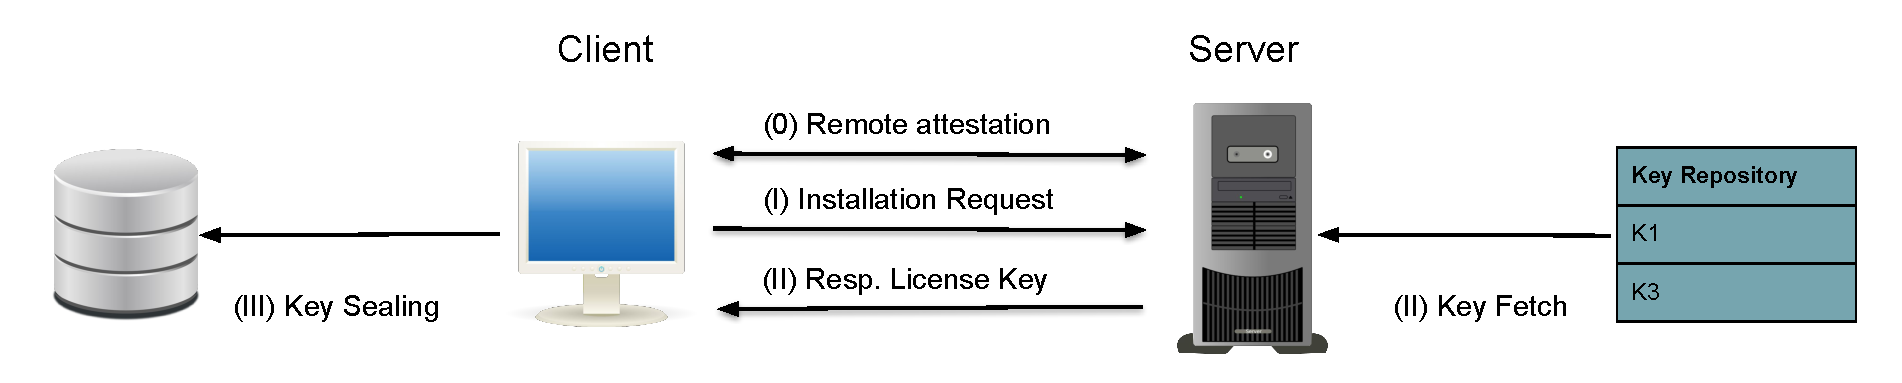
\includegraphics[width=0.9\linewidth]{fig_c3/installation.pdf}
	\caption{Secure installation protocol between client and server.}
	\label{fig:installation}
\end{figure}


%\subsection{Boot phase}
%After the installation phase is concluded, we need a secure license key 
%loading process for a correct client execution.
%%In this implementation, we used the license key also for the encryption and 
%%decryption algorithms, but in other implementations, they might be separated.
%This is guaranteed by SGX sealing feature, after the installation is done, the 
%license key is sealed on the client machine.
%This means that only the client can access that information.
%That is, once the key is loaded inside the enclave it is protected by design.
%In this sense, SGX guarantees confidentiality and integrity to the license key.
%In this context an attacker has mainly three ways to exfiltrate the license 
%key:
%\begin{enumerate*}[label=(\roman*)]
%	\item tampering the enclave,
%	\item using a cover channel,
%	\item exploit the enclave itself.
%\end{enumerate*}
%While the first one is avoided by design, cover channel 
%attacks~\cite{mangard2017malware} 
%and purely exploitations~\cite{swami2017intel,lee2017hacking} are active 
%threats which deserve attention.
%Anyway there are techniques to mitigate cover 
%channels~\cite{zheng2017opaque,shih2017t} and
%the limiting amount of code within the enclave allows developers to avoid bugs 
%like memory corruptions.
%Also, this is only a proof of concept based on SGX.
%The anti-tampering technique described so far and this protocol can be easily 
%re-adapted to other trusted computer technologies that overcome these 
%limitations.

%\subsection{Development Framework}
%\label{ssec:integration}
%\todo{FT: remove it}
%
%In Figure~\ref{fig:lifecycleintegration}, we suggest a development framework 
%which allows a developer to deploy our technique. 
%Ideally, almost all steps we describe should be aggregated in a single 
%compilation phase in a similar fashion then other works 
%like~\cite{shih2017t,seo2017sgx}.
%%However, we opted for this solution because enclave compilation relies on a 
%%proprietary Intel compiler.
%%So, to the best of our knowledge, it is not possible to generate enclave 
%%assembly code by using other open-source compilers like LLVM or G++.
%%\todo{FT: this is not true! I have recently found some works where they 
%%developed LLMV backend for generating SGX bytecode...how do we deal with it?}.
%
%%As suggested in the previous sections, the main idea is to provide a system 
%%which allows one to include our anti-tampering even after a project is 
%%finished.
%In the first step (Figure~\ref{fig:lifecycleintegration}-I), the developer 
%declares which 
%are the critical sections in the source code by using two markers: one for the 
%beginning of the critical section, and another one for its end.
%This is the only manual operation needed.
%After the annotation phase, there is a code-to-code transformation 
%(Figure~\ref{fig:lifecycleintegration}~II) 
%which purpose is two folds:
%\begin{enumerate*}[label=(\roman*)]
%	\item parse the annotated program and check that all critical sections are 
%neither nested nor overlapped,
%	\item include the call functions to the Untrusted DLL.
%\end{enumerate*}
%In this phase, a parser analyzes all critical sections and enumerates them, 
%this will be necessary later for addressing the binary code of the encrypted 
%critical sections.
%At the third phase (Figure~\ref{fig:lifecycleintegration}~III), we employ SGX 
%Intel compiler for emitting the binary code and sign the Trusted DLL (enclave).
%While in the fourth phase (Figure~\ref{fig:lifecycleintegration}-IV), we 
%generate the final
%clients which will be deployed.
%To achieve it, at first we emit as many license keys as many machines we will 
%install the client,
%then, we extract from the program at step (III) the binary code for each 
%critical sections, 
%and, finally, we craft a set of encrypted critical sections by using all 
%license keys.
%In parallel, we save for each license key the respect block table and the 
%encrypted critical sections.
%At the end, for each client, we substitute the critical sections with the 
%encrypted ones.
%At the point, each client and the server have all information for the 
%installation phase previously described.
%The client has the signed enclave and the encrypted critical sections, while 
%the server has
%all licenses keys, block table, and the encrypted critical sections as well.
%For this phase, we used a Python script based on Radare~\cite{radare} to 
%analyzes the code
%and look for the encrypt/decrypt functions defined at step (I).
%%\todo{SJ: shall we briefly summarize why a list of attackers are not feasible 
%%with our design?}
%
%\begin{figure}[t!]
%	\centering
%	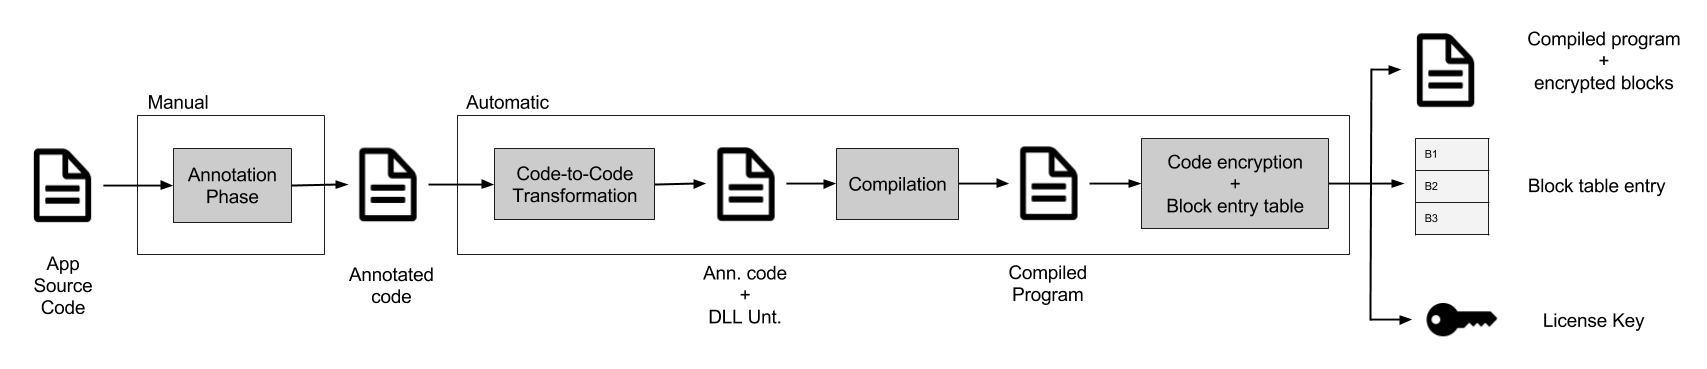
\includegraphics[width=\linewidth]{fig_c3/lifecycleintegration}
%	\caption{Software life-cycle integration}
%	\label{fig:lifecycleintegration}
%\end{figure}

\section{Evaluation}
\label{sec:experiment}

We evaluated our technique from different perspectives.
At first, we quantify the overhead in terms of Lines of Code (LoC), execution 
time (microbenchmark), and memory required by our enclave.
Then, we discuss the impact of several security threats to the infrastructure 
proposed.
Finally, we perform an empirical evaluation of the likelihood to accomplish a 
just-in-time attack.

\subsection{Lines-of-Code Overhead}

A useful metric to measure the impact of our technique is the amount of code 
added to the original program, this is illustrated in Table~\ref{tbl:loc-stats}.
Looking at the table, it is possible to notice that the majority part of the 
code is contained in the main program ($96,5\%$).
The Untrusted and Trusted DLL, which implement our anti-tampering technique, 
require respectively $2,0\%$ and $1,5\%$ of the code.
Within the main program, each CS contains only two lines of code, one for 
calling \texttt{decrypt()} function and another for calling \texttt{encrypt()} 
function.
%These two function calls are automatically appended by using a code-to-code 
%transformation.
We remark that through our technique it is possible to protect an indefinite 
number of CSs by using always the same amount of code in the enclave.
~
\begin{table}[h]
	\center
	\caption{Number of LoC for each module}
	\label{tbl:loc-stats}
	\begin{tabular}{lrr}
		\toprule
		Module & \multicolumn{1}{l}{LoC} & \multicolumn{1}{l}{Perc.} \\
		\midrule
		Main program & 12175 & 96,5\% \\
		Untrusted DLL & 248 & 2,0\% \\
		Trusted DLL & 186 & 1,5\% \\
		\bottomrule
	\end{tabular}
\end{table}

\subsection{Microbenchmark Measurements}
In these experiments, we perform a set of microbenchmark to measure the 
overhead in time introduced by our technique.
As a use case, we measure the execution time of the CSs in our proof-of-concept 
monitoring agent (see Section~\ref{sec:implementation_packing}).
At first, we briefly introduce the experiment setup.
Then, we measure the execution time of the CSs with and without our 
anti-tampering technique.
Finally, we measure the execution time of the CSs in case of multiple instances.
All execution times are measured in milliseconds.

\paragraph{\textbf{User-Simulator Bot}}
For performing the following tests, we developed a user-simulator bot which 
mimics the standard user activity by stroking keys and moving the cursor.
The bot is a Python script which is based on the \emph{PyWin32} library. %for 
%Windows interaction.
Since we aim at measuring the monitoring agent's performances, we designed a 
very basic user-simulator's behavior.
%and not a user's pattern, the user-simulator's behavior is designed to be very 
%simple.
The user-simulator generates keystrokes on a text program (\ie notepad) and 
randomly moves the mouse around the screen.
Keystroke frequency is around $100$ words per minute, while mouse speed is 
around $500$ pixel per second.
This bot allows us to easily repeat the experiments.

%\paragraph{\textbf{Single Instance Anti-Tampering Overhead}}
\paragraph{\textbf{Single Instance Microbenchmark}}
We measure the impact of our anti-tampering technique to the performances of 
the CSs in our proof-of-concept monitoring agent.
In this experiment, we performed $5$ exercises, each of one is composed by two 
runs, namely with and without the anti-tampering technique.
For each run, we traced the CS's execution time.
%We repeat this experiment five times, for $10$ runs in total.
The outcome of the experiment is plotted in 
Figure~\ref{fig:performanceEvaluation}. %and described in 
%Table~\ref{tbl:performance-overhead}.
In the plot, each bar represents the average elapsed time for a run and each 
pair of bars represents a single exercise. More precisely, orange bars
mean runs with the anti-tampering technique active, while blue bars mean runs 
without.
%(no call to any trusted function).
Looking at the graph, we can see that functions require on average between 
$2$ms and $2.4$ms for being executed.
It is also evident that with the anti-tampering technique the performances are 
slightly degraded.
%The delta is well marked in Table~\ref{tbl:performance-overhead}, where rows 
%represent each experiment and columns the relative runs (\ie with and without 
%AT).
On average, the delta time is $0.12$ms, with a peak of $0.34$ms for the second 
instance. 
Also, time overhead is less than $6\%$ on average, with a peak of $16.61\%$ in 
the second instance. 
This peak depends on the system status at execution time.
According to our experiments, we conclude that the performances degradation is 
negligible after the introduction of our anti-tampering system.

\begin{figure}[t]
	\centering
	\begin{subfigure}[t]{0.45\textwidth}
		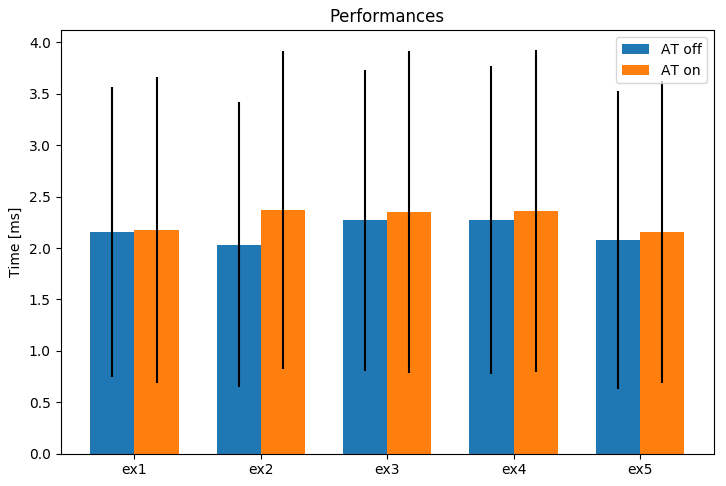
\includegraphics[width=\linewidth]{fig_c3/performanceEvaluation}
		\caption{Average response time with and without anti-tampering 
		technique}
		\label{fig:performanceEvaluation}
	\end{subfigure}
	\hfill
	\begin{subfigure}[t]{0.45\textwidth}
		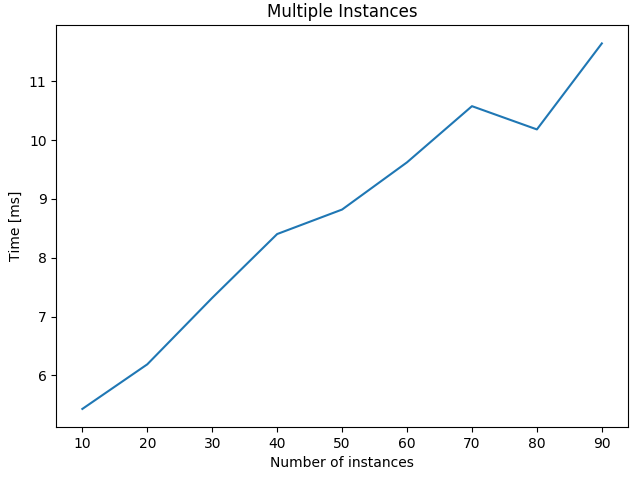
\includegraphics[width=\linewidth]{fig_c3/multiple}
		\caption{Average response time with multiple instances}
		\label{fig:multiple}
	\end{subfigure}
	\caption{Careful-Packing evaluation.}
	\label{fig:performance2}
\end{figure}

\paragraph{\textbf{Multiple Instances}}
We empirically investigate whether our approach can be deployed over multiple 
processes at the same time.
We performed this test by running a different number of instances of our 
proof-of-concept monitoring agent and then measuring the average execution time 
of their CSs.

The outcome of the experiment is depicted in Figure~\ref{fig:multiple}.
The plot shows the average execution time of the CS on the y-axis (expressed in 
milliseconds), while 
the number of instances is indicated on the x-axis (from $10$ to $90$).
Looking at the plot, it is possible to notice that the average execution time 
grows linearly \wrt the number of instances.
The average execution time is around $5$ms in case of $10$ parallel instances, 
while it degrades to $11$ms in case of $90$. 
This means that the performances get only halved after decupling the number of 
instances; therefore, our technique results scalable.
%Moreover, this experiment underlines how our technique manged to protect 90 
%instances contemporaneously.

\subsection{Enclave Size Considerations}
%We measure the trusted container size and we estimate the number of processes 
%we can protect.
In our proof-of-concept monitoring agent, we used an enclave that occupies at 
around $300KB$.
As we stated, in our approach the enclave size does not depend by the size of 
the software to protect.
This allows us to estimate the number of processes we can protect at the same 
time.
%We therefore use the enclave used in our proof-of-concept program to resolve 
%the second point.
In a common machine SGX featured (\eg Dell XPS 13 9370), we can dedicate at 
most $128MB$ for enclaves.
If we consider the enclave used in our proof-of-concept, we can roughly 
estimate at around $400$ enclaves contemporaneously loaded that will protect 
the same number of processes.
%Moreover, we show in the previous paragraph that our technique results 
%scalable over multiple processes.

\subsection{Threat Mitigation}
We explain how our approach mitigates threats according to the attacker model 
described in Section~\ref{ssec:back-attacker}.

\paragraph{\textbf{Protection of checkers and responses.}} In our approach, the 
functions for anti-tampering mechanisms (\eg \emph{checker} and 
\emph{response}) reside in a trusted module. Since we assume trusted computing 
guarantees hardware isolation, those functions are protected by design.

\paragraph{\textbf{Protection against disarm.}}
An attacker can always disarm a function by removing its invocation.
Moreover, SGX is prone to \emph{denial-of-service attacks} due to its nature 
(see Section~\ref{ssec:sgx-core-design}).
We protect trusted invocations by adopting the packaging tactic discussed in 
Section~\ref{sec:approach}.
The software contains parts of code which are encrypted and they need checkers 
action for being executed properly.

\paragraph{\textbf{Just-in-time Patch \& Repair Mitigation}}
%\todo{fact 1: Attackers should sync victim and adversary process  at 100\%. An 
%error implies to be detected.}
%\todo{fact 2: There exists several attempts to tamper a task scheduler (KDON, 
%Okland paper, maybe others), but they do not reach 100\% of sync, indeed, 
%these 
%attacks are more suitable for other scenarios \eg cache attacks, where it is 
%tolerate a bit of noise. Such noise brings to fact 1}
%\todo{fact 3: modern OS (\eg Linux~[cite it]), are designed to resist against 
%common task scheduler attacks}

After a \emph{decryption} function is run, the CS is plain and ready to be 
executed.
At this moment, there is a chance for the attacker to replace the code within a 
CS and restore it before the next \emph{encryption}.
This is called just-in-time patch \& repair attack.

Assuming the attacker cannot directly tamper with the task scheduler (as 
described in Section~\ref{ssec:back-attacker}), it is still possible to perform 
attacks from the user-space~\cite{5958048}.
However, those attacks are not strong enough to bypass our defense for mainly 
three reasons:
\begin{enumerate*}[label=(\roman*)]
	\item they are tailored for specific contexts (\eg single core, OS version),
	\item they aim at slowing down a process and not to achieve a perfect 
	synchronization between adversary and victim,
	\item modern OSs mount task schedulers which are designed to resist (or at 
	least mitigate) such attacks~\cite{cfslinux}.
\end{enumerate*}
To achieve an \emph{on-line} tampering, as introduced in 
Section~\ref{ssec:back-attacker}, an attacker must replace a CS code such that 
\texttt{encrypt()} and \texttt{decrypt()} functions do not notice the 
replacement.
This means that a single error will be detected by the server. 
None of the attacks from user-space can achieve such precision.
An alternative approach is to adopt virtualization to debug a process 
step-by-step at runtime, but this contradicts the assumptions of our threat 
model (\ie the original infrastructure is not altered).
We, however, try to estimate the likelihood that this attack might happen by 
performing an empirical experiment which will be described in 
Section~\ref{sec:just-in-time}.

\paragraph{\textbf{Reverse Engineering}}
An attacker may attempt to reverse the application code in order to extract the 
plain code hidden in the encrypted blocks, and then build a new executable 
which does not contain any checker.
The new executable is therefore prone to any manipulation.
This goal can be achieved by using debuggers and/or analyzers.
Even though the literature contains several anti-debugging techniques and most 
of them can be enforced by using our anti-tampering technique, we assume that 
an attacker can bypass all of them.
However, an attacker cannot debug the software inside the trusted zone, which 
is true for SGX enclaves compiled in release mode~\cite{sgxnodebug}.
The best an attacker can do is debugging the code within the untrusted memory 
region and considering the enclave as a black box.
After applying these considerations, we can state an attacker can manage to 
dump the plain code after that \emph{decryption} functions are called, and even 
make a new custom application.
However, this attack is still coherent with our threat model (see 
Section~\ref{ssec:back-attacker}) because the new application cannot work into 
the original infrastructure (\ie the heartbeat cannot work properly) and 
therefore it is useless.
For instance, in the implementation presented in 
Section~\ref{sec:implementation_packing}, 
the monitoring agent can work properly only if the software contains all the 
functions employed by our technique along with the original CSs.
If this is not respected  (\ie by removing checkers) the application cannot 
emit a correct heartbeat,
and therefore the attack is not considered accomplished.

%We remark that the final goal of this attack is to build a software 
%checker-less which is still useful. The usefulness of this new software 
%depends 
%by the scenario in which it is deployed.
%Therefore, 
%\begin{description}
%	\item[Client with a server interaction] Thanks to \emph{response} function, 
%the heartbeat's signature is wrong and therefore the server can detect the 
%code 
%manipulation.
%	\item[Standalone program which emits output] Even in this case, thanks to 
%the \emph{response} function, an attacker can still use the program but the 
%output is wrongly signed and we can spot the attack.
%	\item[Standalone program without persisten output] Since the software does 
%not emit any result. We cannot detect any manipulation because the 
%\emph{response} function is not used to sign anything and the checkers were 
%removed. Therefore our anti-tampering technique is not suitable for this 
%scenario.
%\end{description}

%\begin{table}[]
%	\centering
%	\caption{Performance overhead table}
%	\label{tbl:performance-overhead}
%	\begin{tabular}{lrrrr}
%		\toprule
%		& \multicolumn{1}{l}{\textbf{AT off}} & \multicolumn{1}{l}{\textbf{AT 
%on}} & \multicolumn{1}{l}{\textbf{$\Delta$ (ms)}} & 
%\multicolumn{1}{l}{\textbf{$\Delta$ (\%)}} \\
%		\midrule
%		ex1 & 2.15 & 2.18 & 0.02 & 0.97\% \\
%		ex2 & 2.03 & 2.37 & 0.34 & 16.61\% \\
%		ex3 & 2.27 & 2.35 & 0.08 & 3.52\% \\
%		ex4 & 2.27 & 2.36 & 0.09 & 3.80\% \\
%		ex5 & 2.08 & 2.15 & 0.07 & 3.58\% \\
%		\midrule
%		\textbf{avg} & \textbf{2.16} & \textbf{2.28} & \textbf{0.12} & 
%\textbf{5.70\%} \\
%		\bottomrule
%	\end{tabular}
%\end{table}

\subsection{Study of Just-in-Time Patch \& Repair Attack}
\label{sec:just-in-time}
In this experiment, we investigate the likelihood of a
just-in-time patch \& repair attack in a real context.
%This experiment is not aimed to investigate all possible attack scenarios, 
%indeed, it is an empirical measurement about the synchronization of two 
%concurrent processes.
Here, the attacker's goal is to temporarily replace the bytecode within a CS 
such that the injected code is executed but the system cannot realize the 
attack.
The setup is formed by a victim process (\ie our agent) and an attacker 
process. %The interaction between attacker and victim is described in 
%Section~\ref{ssec:back-attacker}.
Also, we consider a trusted task scheduler, and that each process is executed 
on a dedicated core.
Both attacker and victim are written in C++ and developed for Windows, the 
experiments were run on a Windows 10 machine with 16GB RAM and 
Intel\textsuperscript{\textregistered} Core\textsuperscript{\texttrademark} 
i7-7500 $2,70$GHz processor.

The victim process is formed by an infinite
loop which continuously updates an internal variable through a CS. This latter 
is enforced by self-checking mechanisms.
Moreover, the victim process contains a checker to validate the status of the 
program. If the internal status is set wrongly, that will be logged.
The attacker process, instead, is a concurrent process which can edit the 
victim process at runtime. Attacker's goal is to replace the victim CS such 
that the internal variable of the victim process will contain an incongruent 
value.
We attempted the attack for $10.000$ times, but the self-checking mechanism 
managed to detect all attacks.
Therefore, we consider that this kind of attack is not practical
in case of a trusted task scheduler.

\section{Discussion}
\label{sec:discussion_packing}

%In this work, we have proposed a set of software protection mechanisms
%that combine anti-tampering techniques and trusted computing 
%(Section~\ref{sec:approach}).
%Our solution hardens both anti-tampering techniques and trusted computed 
%approaches. % (\eg packaging and \emph{denial of service}).
%We also propose solutions to overcome side issues such as secure installation 
%and boot phase.
%In the end, we have deployed our technique in a monitoring agent 
%(Section~\ref{sec:implementation_packing}) and we have empirically shown the 
%scalability of our approach (Section~\ref{sec:experiment}).
We have shown how to implement our technique by means of a case study involving 
a monitor agent, however there are few aspects to note about the validity of 
our evaluation effort.
First, although the application code is protected, 
an attacker can still analyze and change variable values at runtime, thus 
potentially harming its normal execution.
Note that our approach could be extended in order to mitigate this issue by 
using cryptographic hashes to validate the integrity of certain critical 
variables.
%\todo{here}
Moreover, our design and implementation requires a healthy kernel, otherwise it 
would be possible to mount attacks such as the just-in-time patch and repair 
attack we discussed previously (by manipulating the scheduler). We believe  
that even with a compromised kernel mounting those attacks would require 
significant effort, but we leave a more thorough investigation for future work. 
Other aspects, such as an evaluation of applying our technique a different 
granularities (such as basic-block level), or extending protection to 
\emph{PLT}, \emph{GOT}, and \emph{exception table} are also left for future 
work.
%Also, we want to explore new techniques for deploying our solution
%at basic-block level for making the software even more secure and stable.
%Moreover, we want to extend our protection over other binary structure, such 
%as \emph{PLT}, \emph{GOT}, and \emph{exception table}. This can be done by 
%extending the heartbeat functionalities.
%Finally, we want to develop new implementations based on other trusted 
%computing techniques (\eg TPM~\cite{tpm-isoosi}).

%To sum up, to the best of our knowledge, this is the first practical and 
%scalable
%approach which attempts to extend trusted computing features over untrusted 
%zones.
%Thanks to this solution, it is possible to enforce software protection
%with a minimum amount of code within a trusted zone
%and without further monitors or software layers to the original program.